\section{Bayes and Gaussian Processes}

\subsection{Bayes Method}

\begin{remark}{\textbf{(Recap of Bayes)}}
    Model have a parameter $\theta_m$ that specify the probability of data $P(\mathcal{D}|\theta_m, m)$. If the model is known, learning $\theta_m$ means finding a posterior or point estimate. 
    \begin{itemize}
        \item What if we want to learn the type of model too ?
        \item Can we combine the model into a single \correctquote{supermodel} with a composite parameters ? 
        \item We can separate the model selection step: $P(\theta_m,m | \mathcal{D}) = P(\theta_m|m,\mathcal{D})P(m|\mathcal{D})$
    \end{itemize}
\end{remark}

\begin{definition}{\textbf{(Neyman-Peason Hypothesis Testing)}}
    For nested model, starting with simpliest model with $m=1$, comparing null hypothesis $m$ to its alternate $m+1$ and repeat until $m+1$ is rejected. Note that this tests only exact when it is asympototic in data number. Finally, it is conservative as it is asymmetric by design.
\end{definition}

\begin{definition}{\textbf{(Likelihood Validation)}}
    Partition data into disjoint training and validation set, where $D = D_\text{tr}\cup D_\text{valid}$. Then, we choose a model with greatest $P(D_\text{valid} | \theta^\text{ML}_m)$ where:
    \begin{equation*}
        \theta^\text{ML}_m = \argmax{\theta}P(D_\text{tr}|\theta)
    \end{equation*}
    or if we are able to find $P(D_\text{valid}|D_\text{train}, m)$. 
    \begin{itemize}
        \item This model is consistent and select the most useful model even if they are incorrect. 
        \item It may be biased toward a simpler models and gives a high-variance. 
        \item We can use cross-validation is used with multiple partition and average likelihood. 
    \end{itemize}
\end{definition}

\begin{definition}{\textbf{(Baysian Model Selection)}}
    We would like to choose a model $P(m|\mathcal{D})$  where consistent as it is a probability principle if true model is in the set. 
    \begin{itemize}
        \item However, it might be a problem of assumed prior. Finally, the posterior can weights models for combined prediction. 
        \item A model of class $m$ is a set of distributions parameterized by $\theta_m$. The model implies the prior over parameters as the posterior of the parameter:
        \begin{equation*}
            P(\theta_m | \mathcal{D}, m) = \frac{P(\mathcal{D}|\theta_m,m)P(\theta_m|m)}{P(\mathcal{D}|m)} \quad \text{ where } \quad 
        \end{equation*}
        where $P(\mathcal{D}|m)$ is the Baysian evidence for model $m$, where the ratio is known as Bayes factor:
        \begin{equation*}
            \frac{P(\mathcal{D}|m)}{P(\mathcal{D}|m')} = \frac{P(m|\mathcal{D})}{P(m'|\mathcal{D})}\frac{P(m')}{P(m)}
        \end{equation*}
        \item This is linked to Occam's razor where: the model that are \emph{too complex} can generate many data but they can be unlikely to generate a particular dataset. The model that are \emph{too simple} can't generate the data. 
    \end{itemize}
\end{definition}

\begin{remark}{\textbf{(Conjugate Prior)}}
    We will recall the use of exponential model. Suppose, we have $P(\mathcal{D}|\boldsymbol \theta_m,m)$ is member of the exponential family, where we can see that:
    \begin{equation*}
        P(\mathcal{D}|\boldsymbol \theta_m, m) = \prod^N_{i=1}P(\boldsymbol x_i | \boldsymbol \theta_m, m) = \prod^N_{i=1}\exp\bracka{\boldsymbol s(\boldsymbol x_i)^T\boldsymbol \theta_m - A(\boldsymbol \theta_m)}
    \end{equation*}
    Please note that $\boldsymbol A(\boldsymbol \theta_m)$ is the normalizing factor as it is (recall exponential family of the form in previous course) equal to $\ln(g(\boldsymbol \theta_m))$. Consider the prior conjugate to be:
    \begin{equation*}
        P(\boldsymbol \theta | m) = \frac{1}{Z(s_p, n_p)}\exp\bracka{\boldsymbol s_p^T\boldsymbol \theta_m - n_pA(\boldsymbol \theta_m)}
    \end{equation*}
    Then the posterior is equal to:
    \begin{equation*}
        P(\mathcal{D}, \boldsymbol \theta_m | m) = \frac{1}{Z(\boldsymbol s_p, p)}\exp\bracka{\bracka{\sum^N_{i=1}\boldsymbol s(\boldsymbol x_i) + \boldsymbol s_p}^T\boldsymbol \theta_m - (N+n_p)A(\boldsymbol \theta_m)}
    \end{equation*}
    One can show that:
    \begin{equation*}
        P(\mathcal{D}|m) = \int P(\mathcal{D}, \boldsymbol \theta_m | m) \dby\boldsymbol \theta_m = \frac{Z(\sum_i\boldsymbol s(\boldsymbol x_i) + \boldsymbol s_p, N + n_p)}{Z(\boldsymbol s_p, p)}
    \end{equation*}
\end{remark}

\begin{remark}{\textbf{(Laplace Approximation)}}
    To find $P(\mathcal{D} | m)$, we will have to perform the following integration:
    \begin{equation*}
        P(\mathcal{D}|m) = \int P(\mathcal{D}, \boldsymbol \theta_m | m)\dby\boldsymbol \theta_m
    \end{equation*}
    as the datasize $N$ grows, $\boldsymbol \theta$ becomes more concentrated as $P(\mathcal{D}, \boldsymbol \theta_m|m)\propto P(\boldsymbol \theta_m | \mathcal{D}, m)$ becomes concentrated on $\boldsymbol \theta_m^*$. Let's try to approximate the $P(\mathcal{D}, \boldsymbol \theta_m|m)$ to the second order around $\boldsymbol \theta_m^*$:
    \begin{equation*}
    \begin{aligned}
        \int P(\mathcal{D}, \boldsymbol \theta_m|m)\dby\boldsymbol \theta_m &= \int \exp(\log P(\mathcal{D}, \boldsymbol \theta_m|m))\dby \boldsymbol \theta_m \\
        &\approx\begin{aligned}[t]
            \int \exp\Big[ &\log P(\mathcal{D}, \boldsymbol \theta^*_m | m) + \underbrace{\nabla \log P(\mathcal{D}, \boldsymbol \theta_m^* | m)(\boldsymbol \theta_m - \boldsymbol \theta_m^*)}_{0} \\
            &+\frac{1}{2}(\boldsymbol \theta_m-\boldsymbol \theta_m^*)^T\underbrace{\nabla^2\log P(\mathcal{D}, \boldsymbol \theta_m^* | m)}_{-\boldsymbol A}(\boldsymbol \theta_m - \boldsymbol \theta_m^*) \Big]\dby\boldsymbol \theta_m 
        \end{aligned} \\
        &=\int P(\mathcal{D}, \boldsymbol \theta^*_m | m)\exp\brackb{-\frac{1}{2}(\boldsymbol \theta_m-\boldsymbol \theta_m^*)^T\boldsymbol A(\boldsymbol \theta_m - \boldsymbol \theta_m^*)}\dby\boldsymbol \theta \\
        &= P(\mathcal{D}|\boldsymbol \theta^*_m,m)P(\boldsymbol \theta^*_m|m)(2\pi)^{-d/2}\abs{\boldsymbol A}^{-1/2}
    \end{aligned}
    \end{equation*}
    This is approximating the posterior by a Gaussian, where an approximate that is asymmetrically correct. 
\end{remark}

\begin{definition}{\textbf{(Baysian Information Criterion)}}
    BIC can be obtained from Laplace approximate:
    \begin{equation*}
        \log P(\mathcal{D} | m) \approx \log P(\boldsymbol \theta^* | m) + \log P(\mathcal{D}|\boldsymbol \theta^*_m, m) + \frac{d}{2}\log 2\pi - \frac{1}{2}\log\abs{\boldsymbol A}
    \end{equation*}
    where we further have:
    \begin{equation*}
        \boldsymbol A = -\nabla^2\log P(\mathcal{D}, \boldsymbol \theta^*_m | m) = -\nabla^2\log P(\mathcal{D}|\boldsymbol \theta^*, m) -\nabla^2\log P(\boldsymbol \theta^*|m)
    \end{equation*}
    As $N=|D|\rightarrow\infty$ and $A\rightarrow N\boldsymbol A_0 + \text{const}$ for a fixed positive definite matrix $\boldsymbol A_0 = \brackd{-\nabla^2\log P(\boldsymbol x | \boldsymbol \theta^*, m)}$ as we have $\log\abs{N\boldsymbol A_0} = d\log N + \log\abs{\boldsymbol A_0}$. We will retain only the term that grows with $N$ to be:
    \begin{equation*}
        \log P(\mathcal{D} | m) \approx \log P(\mathcal{D}|\boldsymbol \theta^*_m, m) - \frac{d}{2}\log N
    \end{equation*}
\end{definition}

\begin{remark}{\textbf{(Properties BIC)}}
    Baysian Information Criterion has the following properties, as we have:
    \begin{itemize}
        \item Quick and Easy to compute. It doesn't depend on the prior as we can use ML to estimate instead of MAP estimate. 
        \item It is related to minimal description length. Given the assuption that in large sample limit, all parameter are well determined. But it negated multiple nodes (permuation of mixture of Gaussian).
    \end{itemize}
\end{remark}

\begin{definition}{\textbf{(Hyperparameter and Evidence Optimization)}}
    Need to choose between a family of continuous parameterized models:
    \begin{equation*}
        P(\mathcal{D} | \boldsymbol \eta) = \int P(\mathcal{D} | \boldsymbol \theta)P(\boldsymbol \theta | \boldsymbol \eta) \dby \boldsymbol \theta
    \end{equation*}
    We can perform an ascending on gradient in: the exact evidence, approximate evidence (Laplace, BIC) or free-energy based on the evidence (variational Bayes). Performing the hyper-prior on $\boldsymbol \eta$, which we can sample its posterior via MCMC as:
    \begin{equation*}
        P(\boldsymbol \eta | \mathcal{D}) = \frac{P(\mathcal{D}|\boldsymbol \eta)P(\boldsymbol \eta)}{P(\mathcal{D})}
    \end{equation*}
\end{definition}

\subsection{Linear Regression/Gaussian Process}

\begin{definition}{\textbf{(Linear Regression)}}
    We consider the following graphical model as:
    \begin{figure}[H]
        \centering
        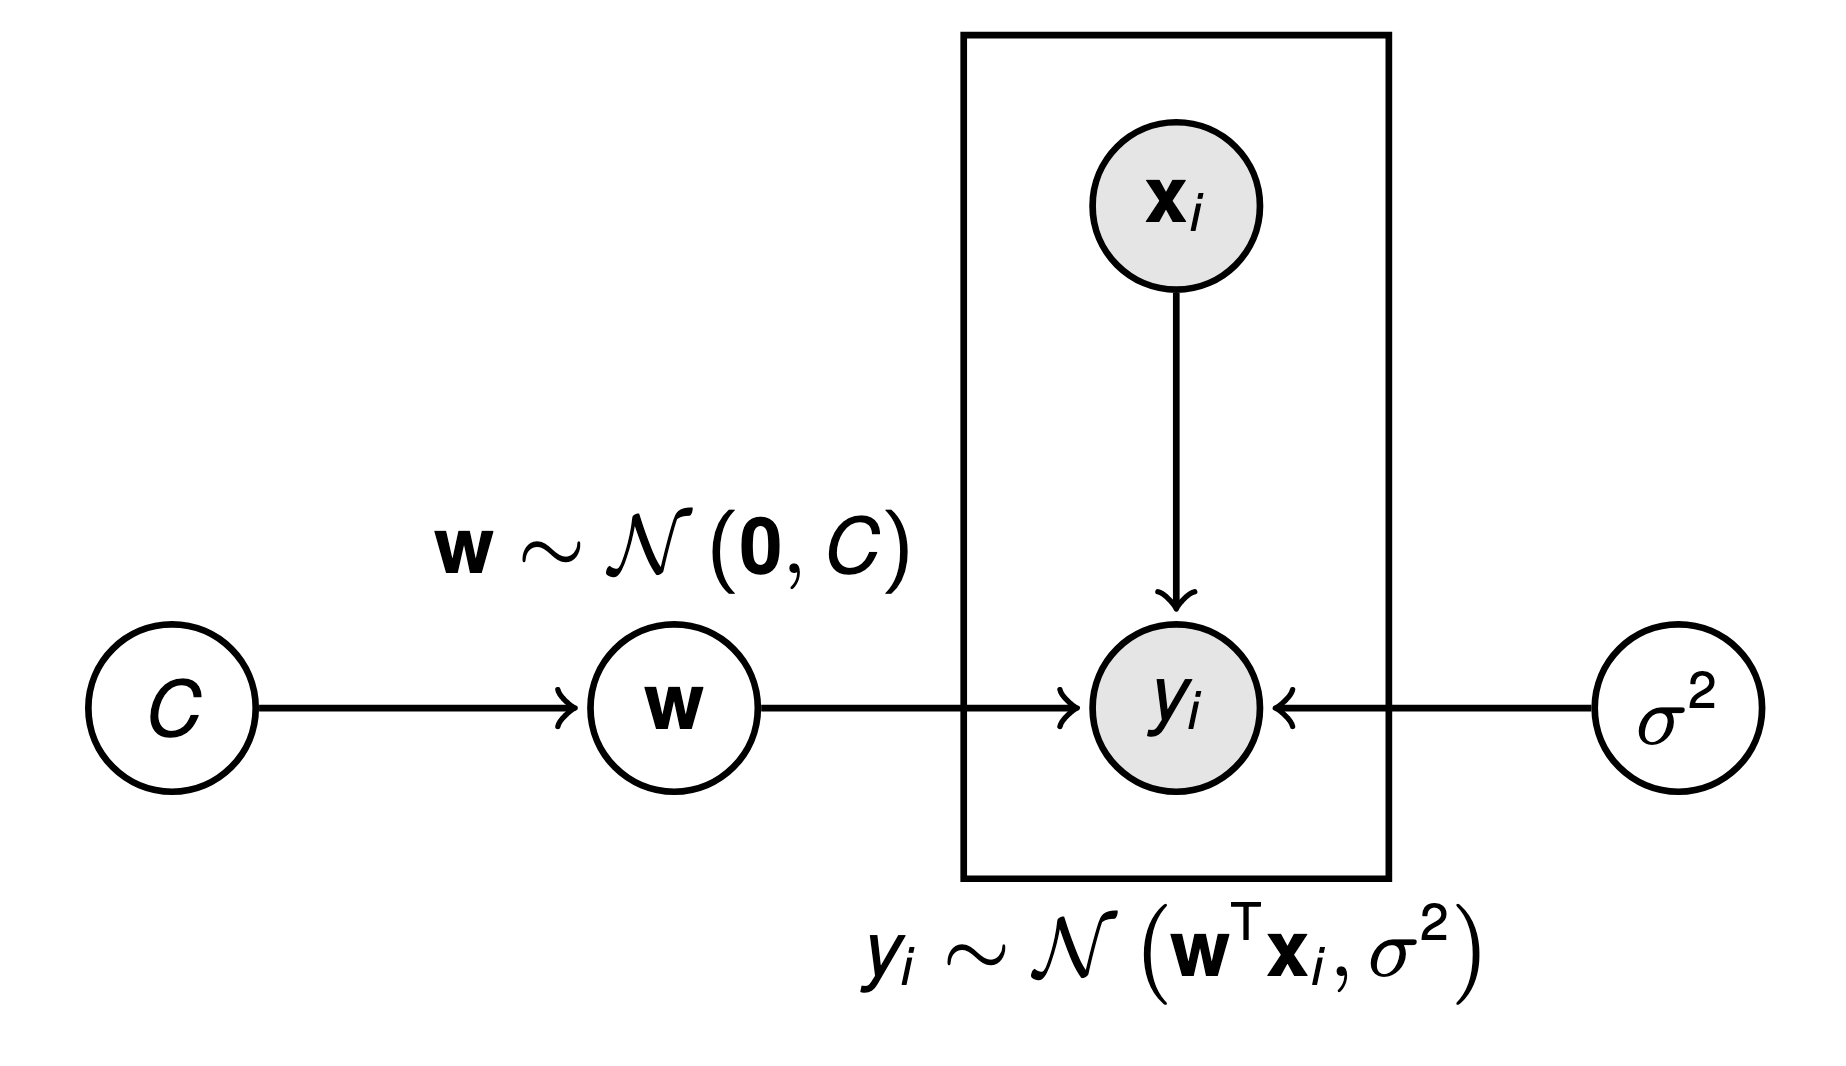
\includegraphics[width=8cm]{img/img11.png}
    \end{figure}  
    To find the hyperparameters, we can see that:
    \begin{equation*}
        P(\brackc{y_i}^N_{i=1} | \brackc{\boldsymbol x_i}^N_{i=1}, \boldsymbol C, \sigma^2) = \int P(\brackc{y_i}^N_{i=1} | \brackc{\boldsymbol x_i}^N_{i=1}, \boldsymbol w, \sigma^2)P(\boldsymbol w | \boldsymbol C)\dby \boldsymbol w
    \end{equation*}
    Maximizing the value of $\boldsymbol C$ and $\sigma^2$.
\end{definition}

\begin{proposition}
    The update rule for the parameter $\boldsymbol \theta = \brackc{\boldsymbol C, \boldsymbol \sigma^2}$ is:
    \begin{equation*}
    \begin{aligned}
        &\frac{\partial}{\partial \boldsymbol \theta} \log \mathcal{E}(\boldsymbol C, \sigma^2) = \frac{1}{2}\operatorname{Tr}\brackb{(\boldsymbol C - \boldsymbol \Sigma_w - \bar{\boldsymbol w}\bar{\boldsymbol w}^T)\frac{\partial}{\partial \boldsymbol \theta} \boldsymbol C^{-1}} \\
        &\frac{\partial}{\partial \sigma^2}\log\mathcal{E}(\boldsymbol C,\sigma^2) = \frac{1}{\sigma^2}\bracka{-N + \operatorname{Tr}[\boldsymbol I - \boldsymbol \Sigma_w\boldsymbol C^{-1}] + \frac{1}{\sigma^2}(\boldsymbol Y - \boldsymbol X^T\bar{\boldsymbol w})^T(\boldsymbol Y - \boldsymbol X^T\bar{\boldsymbol w})}
    \end{aligned}
    \end{equation*}
\end{proposition}

\begin{proof}
    We can see that the posterior of $P\bracka{\boldsymbol w \left| \brackc{y_i}^N_{i=1}, \brackc{\boldsymbol x_i}^N_{i=1}, \boldsymbol C,\sigma^2\right.}$. We can see that the posterior on $\boldsymbol w$ is normal with:
    \begin{equation*}
        \Sigma_{\boldsymbol w} = \bracka{\frac{\boldsymbol X\boldsymbol X^T}{\sigma^2} + \boldsymbol C^{-1}}^{-1} \qquad \bar{\boldsymbol w} = \boldsymbol \Sigma_{\boldsymbol w}\frac{\boldsymbol X\boldsymbol Y}{\sigma^2}
    \end{equation*}
    This follows from the eariler works. Now, we can consider terms inside the exponential of the joint distributions $P(\boldsymbol Y | \boldsymbol X, \boldsymbol w, \sigma^2)P(\boldsymbol w | \boldsymbol C)$:
    \begin{equation*}
    \begin{aligned}
        -\frac{1}{2\sigma^2}\boldsymbol Y^T\boldsymbol Y &+ \frac{1}{\sigma^2}\boldsymbol w^T\boldsymbol X\boldsymbol Y - \frac{1}{2}\Big[ \boldsymbol w^T\boldsymbol \Sigma_w^{-1}\boldsymbol w \Big] \\
        &=-\frac{1}{2\sigma^2}\boldsymbol Y^T\boldsymbol Y - \frac{1}{2}\brackc{\boldsymbol w^T\boldsymbol \Sigma^{-1}_w\boldsymbol w^T - \frac{2}{\sigma^2}\boldsymbol w^T\boldsymbol \Sigma_w\boldsymbol \Sigma^{-1}_w\boldsymbol X\boldsymbol Y} \\
        &=\begin{aligned}[t]
            -\frac{1}{2\sigma^2}\boldsymbol Y^T\boldsymbol Y &- \frac{1}{2}\brackc{\boldsymbol w^T\boldsymbol \Sigma^{-1}_w\boldsymbol w^T - \frac{2}{\sigma^2}\boldsymbol w^T\boldsymbol \Sigma_w\boldsymbol \Sigma^{-1}_w\boldsymbol X\boldsymbol Y + \frac{1}{\sigma^4}\boldsymbol Y^T\boldsymbol X^T\boldsymbol \Sigma^T_w\boldsymbol \Sigma^{-1}_w\boldsymbol \Sigma^T_w\boldsymbol X\boldsymbol Y} \\
            &+ \frac{1}{2\sigma^4}\boldsymbol Y^T\boldsymbol X^T\boldsymbol \Sigma^T_w\boldsymbol X\boldsymbol Y
        \end{aligned} \\
        &= -\frac{1}{2\sigma^2}\boldsymbol Y^T\boldsymbol Y + \frac{1}{2\sigma^4}\boldsymbol Y^T\boldsymbol X^T\boldsymbol \Sigma^T_w\boldsymbol X\boldsymbol Y -\frac{1}{2}\bracka{\boldsymbol w - \frac{1}{\sigma^2}\boldsymbol \Sigma_w\boldsymbol X\boldsymbol Y}^T\boldsymbol \Sigma^{-1}_w\bracka{\boldsymbol w - \frac{1}{\sigma^2}\boldsymbol \Sigma_w\boldsymbol X\boldsymbol Y}
    \end{aligned}
    \end{equation*}
    If we consider the quadratic terms, and the integration over it we have:
    \begin{equation*}
        \int \exp\brackc{-\frac{1}{2}\bracka{\boldsymbol w-\frac{1}{\sigma^2}\boldsymbol \Sigma_w\boldsymbol X\boldsymbol Y}^T\boldsymbol \Sigma^{-1}_w\bracka{\boldsymbol w - \frac{1}{\sigma^2}\boldsymbol \Sigma_w\boldsymbol X\boldsymbol Y}} \dby \boldsymbol w
    \end{equation*}
    This is the Gaussian integration, which it is a constant that we can ignore. This leads to the evidence to be (the normalizing factor can be easily found):
    \begin{equation*}
        \mathcal{E}(\boldsymbol C, \sigma^2) = \sqrt{\frac{\abs{2\pi\boldsymbol \Sigma_w}}{\abs{2\pi\sigma^2\boldsymbol I}\abs{2\pi\boldsymbol C}}}\exp\brackc{-\frac{1}{2}\boldsymbol Y^T\bracka{\frac{I}{\sigma^2} - \frac{\boldsymbol X^T\boldsymbol \Sigma_w\boldsymbol X}{\sigma^4}}\boldsymbol Y}
    \end{equation*}
    Now, let's consider the derivative to be, starting with the value of $\boldsymbol C$, we can see that the relevant values:
    \begin{equation*}
    \begin{aligned}
        \frac{1}{2}\frac{\partial}{\partial \boldsymbol \theta}\log\abs{\boldsymbol \Sigma_w} &- \frac{1}{2}\frac{\partial}{\partial \boldsymbol \theta}\log\abs{\boldsymbol C} + \frac{1}{2}\frac{\partial}{\partial \boldsymbol  \theta}\frac{\boldsymbol Y^T\boldsymbol X^T\boldsymbol \Sigma_w\boldsymbol X\boldsymbol Y}{\sigma^4} \\
        &= -\frac{1}{2}\frac{\partial}{\partial \boldsymbol \theta}\abs{\boldsymbol \Sigma_w^{-1}} + \frac{1}{2}\frac{\partial}{\partial \boldsymbol  \theta}\log\abs{\boldsymbol C^{-1}} + \frac{1}{2}\frac{\partial}{\partial \boldsymbol  \theta}\frac{\boldsymbol Y^T\boldsymbol X^T\boldsymbol \Sigma_w\boldsymbol X\boldsymbol Y}{\sigma^4} \\ 
        &= -\frac{1}{2}\operatorname{Tr}\bracka{\Sigma_w\frac{\partial \boldsymbol C^{-1}}{\partial \boldsymbol \theta}} + \frac{1}{2}\operatorname{Tr}\bracka{\boldsymbol C\frac{\partial \boldsymbol C^{-1}}{\partial \boldsymbol \theta}} + \frac{1}{2\sigma^4}\operatorname{Tr}\bracka{\boldsymbol X\boldsymbol Y\boldsymbol Y^T\boldsymbol X^T\frac{\partial \boldsymbol \Sigma^{-1}_w}{\partial \boldsymbol \theta}} \\
        &=\begin{aligned}[t]
            -\frac{1}{2}\operatorname{Tr}&\bracka{\Sigma_w\frac{\partial \boldsymbol C^{-1}}{\partial \boldsymbol \theta}} + \frac{1}{2}\operatorname{Tr}\bracka{\boldsymbol C\frac{\partial \boldsymbol C^{-1}}{\partial \boldsymbol \theta}} \\
            &- \frac{1}{2\sigma^4}\operatorname{Tr}\bracka{\boldsymbol X\boldsymbol Y\boldsymbol Y^T\boldsymbol X^T \boldsymbol \Sigma^{-1}_w\frac{\partial}{\partial \boldsymbol \theta}\brackb{ \frac{\boldsymbol X\boldsymbol X^T}{\sigma^2} + \boldsymbol C^{-1}}\boldsymbol \Sigma_w} \\
        \end{aligned}  \\
        &=\begin{aligned}[t]
            -\frac{1}{2}\operatorname{Tr}&\bracka{\Sigma_w\frac{\partial \boldsymbol C^{-1}}{\partial \boldsymbol \theta}} + \frac{1}{2}\operatorname{Tr}\bracka{\boldsymbol C\frac{\partial \boldsymbol C^{-1}}{\partial \boldsymbol \theta}} \\
            &- \frac{1}{2\sigma^4}\operatorname{Tr}\bracka{\boldsymbol X\boldsymbol Y\boldsymbol Y^T\boldsymbol X^T \boldsymbol \Sigma_w\brackb{ \frac{\partial\boldsymbol C^{-1}}{\partial \boldsymbol \theta} }\boldsymbol \Sigma_w} \\
        \end{aligned}  \\
        &=\begin{aligned}[t]
            -\frac{1}{2}\operatorname{Tr}&\bracka{\Sigma_w\frac{\partial \boldsymbol C^{-1}}{\partial \boldsymbol \theta}} + \frac{1}{2}\operatorname{Tr}\bracka{\boldsymbol C\frac{\partial \boldsymbol C^{-1}}{\partial \boldsymbol \theta}} \\
            &- \frac{1}{2}\operatorname{Tr}\bracka{\frac{\boldsymbol Y^T\boldsymbol X^T \boldsymbol \Sigma_w}{\sigma^2}\brackb{ \frac{\partial\boldsymbol C^{-1}}{\partial \boldsymbol \theta} }\frac{\boldsymbol \Sigma_w\boldsymbol X\boldsymbol Y}{\sigma^2}} \\
        \end{aligned}  \\
        &=\begin{aligned}[t]
            -\frac{1}{2}\operatorname{Tr}&\bracka{\Sigma_w\frac{\partial \boldsymbol C^{-1}}{\partial \boldsymbol \theta}} + \frac{1}{2}\operatorname{Tr}\bracka{\boldsymbol C\frac{\partial \boldsymbol C^{-1}}{\partial \boldsymbol \theta}} - \frac{1}{2}\operatorname{Tr}\bracka{\bar{\boldsymbol w}\bar{\boldsymbol w}^T\brackb{ \frac{\partial\boldsymbol C^{-1}}{\partial \boldsymbol \theta} }} \\
        \end{aligned} 
    \end{aligned}
    \end{equation*}
    Please recall the derivative of the inverse, and we finish the proof. Now consider the derivative of the evidence with respected to $S = \sigma^2$, 
    \begin{equation*}
    \begin{aligned}
        \underbrace{\frac{1}{2}\frac{\partial}{\partial S}\log\abs{\boldsymbol \Sigma_w}}_{\circled{1}} &- \frac{N}{2}\frac{\partial }{\partial S} \log S -\frac{1}{2}\frac{\partial }{\partial S}\frac{\boldsymbol Y^T\boldsymbol Y}{S} + \underbrace{\frac{1}{2}\frac{\partial }{\partial S}\frac{\boldsymbol Y^T\boldsymbol X^T\boldsymbol \Sigma_w\boldsymbol X\boldsymbol Y}{S^2} }_{\circled{2}}
    \end{aligned}
    \end{equation*}
    And we have the following derivative for $\circled{1}$, as we have:
    \begin{equation*}
    \begin{aligned}
        \frac{\partial}{\partial S}\log\abs{\boldsymbol \Sigma_w} &= -\frac{\partial}{\partial S}\log\abs{\boldsymbol \Sigma_w^{-1}} \\
        &=- \operatorname{Tr}\bracka{\boldsymbol \Sigma_w\frac{\partial \boldsymbol \Sigma_w^{-1}}{\partial S}} \\
        &=- \operatorname{Tr}\bracka{\boldsymbol \Sigma_w\frac{\partial}{\partial S}\brackb{\frac{\boldsymbol X\boldsymbol X^T}{S} + \boldsymbol C^{-1}}} \\
        &=\frac{1}{S^2} \operatorname{Tr}\bracka{\boldsymbol \Sigma_w\boldsymbol X\boldsymbol X^T} \\
    \end{aligned}
    \end{equation*}
    For for the equation $\circled{2}$, we have:
    \begin{equation*}
    \begin{aligned}
        \frac{\partial }{\partial S}\frac{\boldsymbol Y^T\boldsymbol X^T\boldsymbol \Sigma_w\boldsymbol X\boldsymbol Y}{S^2} &= \boldsymbol Y^T\boldsymbol X^T\boldsymbol \Sigma_w\boldsymbol X\boldsymbol Y\frac{\partial }{\partial S}\frac{1}{S^2} + \frac{1}{S^2}\frac{\partial }{\partial S}\boldsymbol Y^T\boldsymbol X^T\boldsymbol \Sigma_w\boldsymbol X\boldsymbol Y \\
        &= -2\frac{\boldsymbol Y^T\boldsymbol X^T\boldsymbol \Sigma_w\boldsymbol X\boldsymbol Y}{S^3} + \frac{1}{S}\boldsymbol Y^T\boldsymbol X^T\boldsymbol \Sigma_w\frac{\partial }{\partial S}\brackb{\frac{\boldsymbol X\boldsymbol X^T}{S} + C^{-1}}\frac{1}{S}\boldsymbol \Sigma_w\boldsymbol X\boldsymbol Y \\
        &= -2\boldsymbol Y^T\boldsymbol X^T\bar{\boldsymbol w} + \bar{\boldsymbol w}^T \bracka{\boldsymbol X\boldsymbol X^T}\bar{\boldsymbol w}
    \end{aligned}
    \end{equation*}
    Combining them and we have:
    \begin{equation*}
    \begin{aligned}
        \frac{1}{2S}\Bigg( &\frac{1}{S}\operatorname{Tr}\bracka{\boldsymbol \Sigma_w\boldsymbol X\boldsymbol X^T} - N + \frac{1}{S}\boldsymbol Y^T\boldsymbol Y - \frac{1}{S}2\boldsymbol Y^T\boldsymbol X^T\bar{\boldsymbol w} + \frac{1}{S}\bar{\boldsymbol w}^T \Sigma_w\bracka{\boldsymbol X\boldsymbol X^T}\bar{\boldsymbol w} \Bigg) \\
        &= \frac{1}{2S}\bracka{-N + \frac{1}{S}\operatorname{Tr}\bracka{ \boldsymbol \Sigma_w\boldsymbol X\boldsymbol X^T} + \frac{1}{S} (\boldsymbol Y - \boldsymbol X^T\bar{\boldsymbol w})^T(\boldsymbol Y - \boldsymbol X^T\bar{\boldsymbol w}) }
    \end{aligned}
    \end{equation*}
    Please note that there are some differeces between this and the final proof, which we can't get it but most of them seem correct already
\end{proof}

\begin{definition}{\textbf{(Automatic Relevence Determination (ARD))}}
    The most common form of evidence optimization with $\boldsymbol C^{-1} = \operatorname{diag}(\boldsymbol \alpha)$ and the optimize $\{\alpha_i\}$ setting the gradient to $0$, which we now have:
    \begin{equation*}
        \alpha^\text{new}_i = \frac{1-\alpha_i[\boldsymbol \Sigma_n]_{ii}}{\bar{w}_i^2} \qquad (\alpha^2)^\text{new} = \frac{(\boldsymbol Y - \boldsymbol X^T\bar{\boldsymbol w})^T(\boldsymbol Y - \boldsymbol X^T\bar{\boldsymbol w})}{N - \sum_i (1 - [\boldsymbol \Sigma_w]_{ii}\alpha_i)}
    \end{equation*}
    During the optimization, there are $2$ possible scenario for $\boldsymbol \alpha$:
    \begin{itemize}
        \item $\alpha_i\rightarrow\infty$ where the weight $\alpha_i = 0$
        \item $\alpha_i$ is finite and so $w_i = \arg\max P(w_i | \boldsymbol X, \boldsymbol Y, \alpha_i)$
    \end{itemize}
    This is called Automatic Relevence Determination (ARD), which yields space solution that improve ML regression (like LASSA) This Evidence maximization is called ML likelihood or ML-2. 
\end{definition}

\begin{definition}{\textbf{(Prediction Averaging)}}
    We integrate out the parameter, where we have the density estimation:
    \begin{equation*}
        P(\boldsymbol x | \mathcal{D}, m) = \int P(\boldsymbol x | \boldsymbol \theta, m)P(\boldsymbol \theta | \mathcal{D}, m)\dby \boldsymbol \theta
    \end{equation*} 
    Or, perform the prediction:
    \begin{equation*}
        P(y | \boldsymbol x, \mathcal{D}, m) =\int P(y | \boldsymbol x, \theta, m)P(\theta|\mathcal{D}, m)\dby\boldsymbol \theta
    \end{equation*}
    This kind of prediction might resists overfitting with infintely complex model as this can be called Baysian non-parametric, which leads to Gaussian Process.
\end{definition}

\begin{proposition}{\textbf{(Prediction)}}
    Given a new input vector $\boldsymbol x$, the predicted output $y$ is given by:
    \begin{equation*}
        y | \boldsymbol x \sim \mathcal{N}(\bar{\boldsymbol w}^T\boldsymbol x, \boldsymbol x^T\boldsymbol \Sigma_w\boldsymbol x + \sigma^2)
    \end{equation*}
    This comes from the linear Gaussian model. The variance $\boldsymbol x^T\boldsymbol \Sigma_w\boldsymbol x$ that comes from the uncertainty of $\boldsymbol w$.
\end{proposition}

\begin{remark}{\textbf{(Observation on Joint Distribution)}}
    Consider the joint probability between $y_1,\dots,y_N$ and $\boldsymbol x_1, \dots,\boldsymbol x_N$, and noisy prediction with variance $\tau^2$, we can see that the mean and the covariances are:
    \begin{equation*}
    \begin{aligned}
        &\mathbb{E}[y_i] = \mathbb{E}[\boldsymbol w^T\boldsymbol x_i] = 0 \\
        &\mathbb{E}[(y_i-\bar{y}_i)^2] = \mathbb{E}[(\boldsymbol x_i^T\boldsymbol w)(\boldsymbol w^T\boldsymbol x_i)] + \sigma^2 = \tau^2\boldsymbol x_i^T\boldsymbol x_i + \sigma^2 \\
        &\mathbb{E}[(y_i-\bar{y}_i)(y_j-\bar{y}_j)] = \mathbb{E}[(\boldsymbol x_i^T\boldsymbol w)(\boldsymbol w^T\boldsymbol x_j)] = \tau^2 \boldsymbol x_i^T\boldsymbol x_j
    \end{aligned}
    \end{equation*}
    So the leads to the following joint distributions:
    \begin{equation*}
        \left.\begin{bmatrix}
            y_1 \\ y_2 \\ \vdots \\ y_N
        \end{bmatrix}\right| \boldsymbol x_1,\dots,\boldsymbol x_N \sim \mathcal{N}\bracka{\begin{bmatrix}
            0 \\ 0 \\ \vdots \\ 0
        \end{bmatrix}, \begin{bmatrix}
            \tau^2\boldsymbol x_1^T\boldsymbol x_1 + \sigma^2 & \tau^2\boldsymbol x_1^T\boldsymbol x_2 & \cdots & \tau^2\boldsymbol x_1^T\boldsymbol x_N \\
            \tau^2\boldsymbol x_2^T\boldsymbol x_1 & \tau^2\boldsymbol x_2^T\boldsymbol x_2 + \sigma^2 & \cdots & \tau^2\boldsymbol x_2^T\boldsymbol x_N \\
            \vdots & \vdots & \ddots & \vdots \\
            \tau^2\boldsymbol x_N^T\boldsymbol x_1 & \tau^2\boldsymbol x_N^T\boldsymbol x_2 & \cdots & \tau^2\boldsymbol x_N^T\boldsymbol x_N + \sigma^2  \\
        \end{bmatrix}}
    \end{equation*}
    If we were to consider adding the test input vector $\boldsymbol x$ and test vector $y$, we have:
    \begin{equation*}
        \left.\begin{bmatrix}
            \boldsymbol Y^T \\ y
        \end{bmatrix}\right| \boldsymbol X, \boldsymbol x \sim \mathcal{N}\bracka{\begin{bmatrix}
            \boldsymbol 0 \\ 0
        \end{bmatrix}, \begin{bmatrix}
            \tau \boldsymbol X^T\boldsymbol X + \sigma^2\boldsymbol I & \tau^2 \boldsymbol X^T\boldsymbol x \\
            \tau^2 \boldsymbol x^T\boldsymbol X & \tau \boldsymbol x^T\boldsymbol x + \sigma^2
        \end{bmatrix}} = \mathcal{N}\bracka{\begin{bmatrix}
            \boldsymbol 0 \\ 0
        \end{bmatrix}, \begin{bmatrix}
            \tilde{\boldsymbol K}_{XX} & \tilde{\boldsymbol K}_{Xx} \\
            \tilde{\boldsymbol K}_{xX} & \tilde{\boldsymbol K}_{xx} \\
        \end{bmatrix}}
    \end{equation*}
    By the linear Gaussian model, we are given, the following conditional
    \begin{equation*}
    \begin{aligned}
        y | \boldsymbol Y, \boldsymbol X, \boldsymbol x &\sim \mathcal{N}\Big( \tilde{\boldsymbol K}_{xX}\tilde{\boldsymbol K}_{XX}^{-1}\boldsymbol Y^T, \ \tilde{\boldsymbol K}_{xx} - \tilde{\boldsymbol K}_{xX}\tilde{\boldsymbol K}_{XX}^{-1}\tilde{\boldsymbol K}_{Xx} \Big) \\
        &\sim \mathcal{N}\Big( \tau^2\boldsymbol x^T\boldsymbol X(\tau^2 \boldsymbol X^T\boldsymbol X + \sigma^2 \boldsymbol I)^{-1}\boldsymbol Y^T, \ \tau^2\boldsymbol x^T\boldsymbol x + \sigma^2 - \tau^2\boldsymbol x^T\boldsymbol X(\tau^2\boldsymbol X^T\boldsymbol X + \sigma^2)^{-1}\tau^2\boldsymbol X^T\boldsymbol x \Big) \\
        &\sim \mathcal{N}\bracka{ \boldsymbol x^T\frac{1}{\sigma^2} \boldsymbol \Sigma\boldsymbol X\boldsymbol Y^T, \boldsymbol x^T\boldsymbol \Sigma\boldsymbol x + \sigma^2 }
    \end{aligned}
    \end{equation*}
    where $\boldsymbol \Sigma = (\frac{1}{\sigma^2}\boldsymbol X\boldsymbol X^T + \frac{1}{\tau^2}\boldsymbol I)^{-1}$. The derivation comes from the Woodbury identity. 
\end{remark}

\begin{remark}{\textbf{(Non-Linear Regression)}}
    We consider the mapping $\boldsymbol x\mapsto \boldsymbol \phi(\boldsymbol x)$, the regression:
    \begin{equation*}
        \boldsymbol Y | \boldsymbol X \sim \mathcal{N}(\boldsymbol 0_N, \tau^2 \boldsymbol \Phi^T\boldsymbol \Phi + \sigma^2\boldsymbol I_N)
    \end{equation*}
    where $i$-th column of matrix $\boldsymbol \Phi$ is $\boldsymbol \phi(\boldsymbol x_i)$. Now we have the following prediction:
    \begin{equation*}
        \boldsymbol y | \boldsymbol Y, \boldsymbol X, \boldsymbol x \sim \mathcal{N}(\tilde{\boldsymbol K}_{xX}\tilde{\boldsymbol K}_{XX}^{-1}\boldsymbol Y^T, \ \tilde{\boldsymbol K}_{xx}-\tilde{\boldsymbol K}_{xX}\tilde{\boldsymbol K}^{-1}_{XX}\tilde{\boldsymbol K}_{Xx})
    \end{equation*}
    where we have:
    \begin{equation*}
        \tilde{\boldsymbol K}_{XX} = \tau^2\boldsymbol \Phi^T\boldsymbol \Phi + \sigma^2\boldsymbol I \qquad \tilde{\boldsymbol K}_{Xx} = \tau^2\boldsymbol \Phi^T\boldsymbol \phi(\boldsymbol x) \qquad \tilde{\boldsymbol K}_{xx} = \tau^2\boldsymbol \phi(\boldsymbol x)^T\boldsymbol \phi(\boldsymbol x) + \sigma^2
    \end{equation*}
\end{remark}

\begin{remark}{\textbf{(Kernel Vector)}}
    Define a covariance kernel function $\tilde{K}:\mathbb{X}\times \mathbb{X}\rightarrow \mathbb{R}$ if $\boldsymbol x, \boldsymbol x' \in \mathbb{X}$ are $2$ inputs vectors with corresponding output $y$ and $y'$, then we have:
    \begin{equation*}
        \tilde{K}(\boldsymbol x,\boldsymbol x') = \operatorname{Cov}[y, y'] = \mathbb{E}[yy'] - \mathbb{E}[y]\mathbb{E}[y']
    \end{equation*}
    In non-linear regression problem we have $\tilde{K}(\boldsymbol x, \boldsymbol x') =\tau^2\boldsymbol \phi(\boldsymbol x)^T\boldsymbol \phi(\boldsymbol x') + \sigma^2\delta[\boldsymbol x = \boldsymbol x']$, where the prediction depends on $\tilde{\boldsymbol K}(\boldsymbol x, \boldsymbol x')$ rather than its feature map $\boldsymbol \phi(\boldsymbol x)$ and so, we have:
    \begin{equation*}
        \boldsymbol Y | \boldsymbol X, \tilde{\boldsymbol K} \sim \mathcal{N}(\boldsymbol 0_N, \tilde{\boldsymbol K}_{XX})
    \end{equation*}
    To perform a prediction, as we have:
    \begin{equation*}
        \boldsymbol y | \boldsymbol Y, \boldsymbol X, \boldsymbol x \sim \mathcal{N}(\tilde{\boldsymbol K}_{xX}\tilde{\boldsymbol K}_{XX}^{-1}\boldsymbol Y^T, \ \tilde{\boldsymbol K}_{xx}-\tilde{\boldsymbol K}_{xX}\tilde{\boldsymbol K}^{-1}_{XX}\tilde{\boldsymbol K}_{Xx})
    \end{equation*}
    where $\brackb{\tilde{\boldsymbol K}_{XX}}_{ij} = \tilde{\boldsymbol K}(\boldsymbol x_i, \boldsymbol x_j)$, $\brackb{\tilde{\boldsymbol K}_{Xx}}_i = \tilde{\boldsymbol K}(\boldsymbol x_i, \boldsymbol X)$ and $\tilde{K}_{xx} = \tilde{\boldsymbol K}(\boldsymbol x, \boldsymbol x)$, now we can have the kernel function solely without the use of the feature map. 
\end{remark}

\begin{definition}{\textbf{(Gaussian Process)}}
    Let $f(\boldsymbol x)$ be random variable indexed by $\boldsymbol x$, then drawn from the whole GP, which is a random function $f:\mathbb{X}\rightarrow \mathbb{R}$ where:
    \begin{equation*}
        f(\cdot) \sim \mathcal{GP}(m(\cdot), k(\cdot, \cdot))
    \end{equation*}
    It is defiend such that the finite list of points $\brackc{\boldsymbol x_1,\dots,\boldsymbol x_N}$. The joint distributions of the function value $f=[f(\boldsymbol x_1),\dots,f(\boldsymbol x_N)]^T$ as we have $\boldsymbol f | \boldsymbol X, \boldsymbol K \sim \mathcal{N}(\boldsymbol m, \boldsymbol K_{XX})$ with the following parameters:
    \begin{equation*}
        [\boldsymbol K_{XX}]_{ij} = K(\boldsymbol x_i, \boldsymbol x_j) \qquad [\boldsymbol m]_i = \boldsymbol m(\boldsymbol x_i)
    \end{equation*}
\end{definition}

\begin{remark}{\textbf{(Properties of Gaussian Process + Bayes Theorem)}}
    If we assume the random function is dranw from GP prior $f(\cdot) \sim \mathcal{GP}(\boldsymbol 0, K(\cdot, \cdot))$. Observation $y_i$ taken to be noisy version of latent function $f(\boldsymbol x_i)$ where we have:
    \begin{equation*}
        \boldsymbol y_i | \boldsymbol x_i, f(\cdot) \sim \mathcal{N}(y(\boldsymbol x_i), \sigma^2)
    \end{equation*}
    The we have the following quantities:
    \begin{itemize}
        \item The latent $f$ is also Gaussian process:
        \begin{equation*}
            f(\cdot) | \boldsymbol X, \boldsymbol Y \sim \mathcal{GP}\Big( \boldsymbol K_{\cdot X}(\boldsymbol K_{XX} + \sigma^2I)^{-1}\boldsymbol Y^T, \ K(\cdot,\cdot) - K_{\cdot X}(\boldsymbol K_{XX} + \sigma^2\boldsymbol I)^{-1}\boldsymbol K_{X\cdot} \Big)
        \end{equation*}
        \item This is given multivariate Gaussian likelihood:
        \begin{equation*}
            P(\boldsymbol Y | \boldsymbol X) = \abs{2\pi(\boldsymbol K_{xx} + \sigma^2\boldsymbol I)^{-1/2}}\exp\bracka{-\frac{1}{2}\boldsymbol Y(\boldsymbol K_{xx} + \sigma^2\boldsymbol I)\boldsymbol Y^T}
        \end{equation*}
        \item The posterior of $f$ with observation noise, as we have:
        \begin{equation*}
            y | \boldsymbol X, \boldsymbol Y, \boldsymbol x \sim \mathcal{N}(\mathbb{E}[f(\boldsymbol x) | \boldsymbol X, \boldsymbol Y], \operatorname{Var}[f(\boldsymbol x) | \boldsymbol X, \boldsymbol Y] + \sigma^2)
        \end{equation*}
    \end{itemize}
\end{remark}



